\subsection*{Contextual acceptability of complete messages}\label{sec:v4-contextual-results}\label{sec:v4-results}
All three judges accepted the six clear and six minor-imperfection calibration messages. Llama and Mistral rejected five of six constructed disruptions and Qwen rejected six. The two missed contradictions remain in the calibration record. This check supports basic rubric interpretation, not human validity. No rubric amendment was made.

The full frozen sample contains 576 encoded messages from 288 trials and 48 payloads, including 85 messages unavailable under the old window rules. Using 537 complete pairs, the equally weighted panel accepts 90.3 [88.4, 92.1]\% of encoded messages and 96.6 [95.0, 98.1]\% of matched greedy ordinary messages. The paired difference is -6.3 [-8.7, -3.9] percentage points. Brackets denote 95\% payload-cluster intervals conditional on paired availability. The Mistral-source difference interval includes zero, which does not establish equivalence. Table~\ref{tab:v4-contextual} and Fig.~\ref{fig:v4-contextual} show the overall and generator-specific estimates.

\begin{table}[H]\centering\small
\begin{tabular}{lrrrrrr}\toprule
Source & Pairs & RankCloak & Ordinary & Difference & \multicolumn{2}{c}{Disagreement}\\
 & & \% [95\% CI] & \% [95\% CI] & pp [95\% CI] & Enc.\% & Ord.\%\\\midrule
Panel overall & 537 & \shortstack{90.3\\{}[88.4, 92.1]} & \shortstack{96.6\\{}[95.0, 98.1]} & \shortstack{-6.3\\{}[-8.7, -3.9]} & 14.6 & 6.7\\
Llama & 182 & \shortstack{91.1\\{}[87.0, 94.8]} & \shortstack{100.0\\{}[100.0, 100.0]} & \shortstack{-8.9\\{}[-13.0, -5.2]} & 7.3 & 0.0\\
Mistral & 191 & \shortstack{87.8\\{}[84.1, 91.2]} & \shortstack{92.7\\{}[88.8, 96.1]} & \shortstack{-4.9\\{}[-9.9, 0.3]} & 23.4 & 14.6\\
Qwen & 164 & \shortstack{92.3\\{}[89.1, 95.1]} & \shortstack{98.1\\{}[95.9, 99.7]} & \shortstack{-5.9\\{}[-9.1, -2.7]} & 13.0 & 3.7\\
\bottomrule\end{tabular}
\caption{Intact-message contextual acceptability. Acceptance is disruption level 0 or 1. The equally weighted two-judge panel is averaged within trial and payload. The selected sample contains 48 payload clusters, with 288 trials overall and 96 per generator. Pairs counts complete panel-paired messages. Paired percentile intervals use 2,000 class-stratified payload draws and condition on the fixed greedy controls. The Qwen row has 47 observed payload clusters. Disagreement uses the same hierarchy on available pairs of judges within each arm, with 562 encoded and 551 ordinary messages overall. These are automated ratings, not human reading outcomes.}\label{tab:v4-contextual}
\end{table}


\begin{figure}[H]
\centering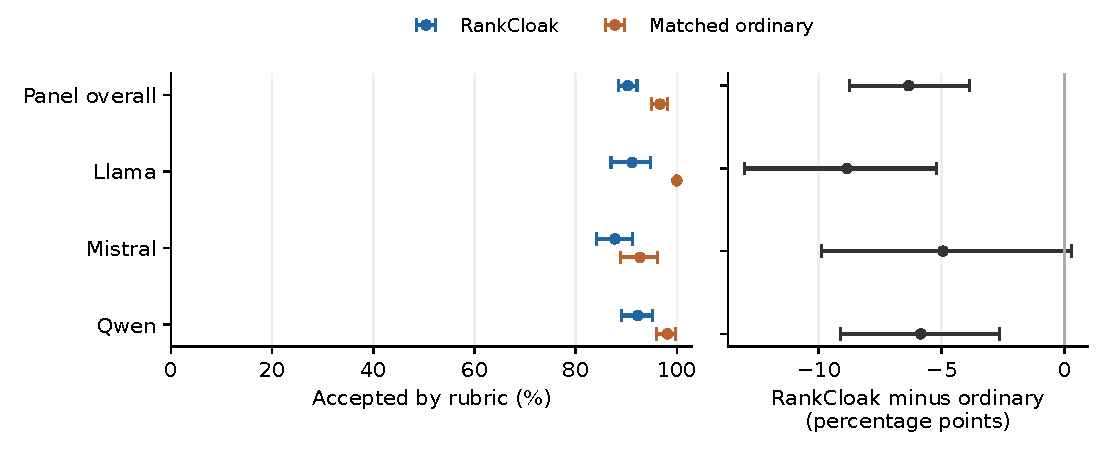
\includegraphics[width=\textwidth]{figures/contextual_acceptability.pdf}
\caption{\textbf{Automated acceptability of intact messages.} The two-judge panel applies the same lenient rubric to RankCloak and matched greedy ordinary output. Left, acceptance at disruption levels 0 or 1. Right, the paired difference in percentage points. Error bars are 95\% intervals from 2,000 class-stratified payload-cluster draws. Intervals condition on the fixed control set. Generator rows use different pairs of judges, so generator and judge effects are not fully crossed. These are automated judgments, not human acceptance or detection rates.}\label{fig:v4-contextual}
\end{figure}

Mean logical connectedness is 3.60 [3.53, 3.67]/5 for encoded messages and 4.00 [3.94, 4.06]/5 for ordinary messages. Binary judge disagreement is 14.6\% and 6.7\%, respectively. The panel distribution over levels 0, 1, 2 and 3 is 11.5, 78.8, 8.5 and 1.2\% for encoded messages. Full distributions for both arms, individual judges, both schedules and realized lengths appear in Supplementary Note S20. The 1,182 unique requests supply 2,304 mapped assignments, with 20 invalid final responses and 31 retries. The primary panel uses 537 complete pairs in 280 trials, retaining all 48 payload clusters. Assigning every missing encoded score as disrupted or acceptable gives an all-slot acceptance range of 88.9 to 90.5\%. Corresponding ordinary bounds are 94.8 to 97.0\%, with a paired difference from -8.1 to -4.3 percentage points. These sensitivity bounds are not confidence intervals. No missing score is treated as acceptance.

Across all valid encoded judgments, 110 are disrupted. Of these, 104 contain a literal passage and 73 quote across the recorded boundary. This post-scoring mapping is descriptive. Whole-message quotations may cross a boundary incidentally. It neither attributes a defect causally to the boundary nor treats an absent quotation as absence of a defect. Identity-selected full-message examples include agreement on acceptance, disagreement and agreement on disruption where available. The earlier fragment pilots and limited fixed-path likelihood findings remain in Supplementary Note S17.


\subsection*{Mechanisms of transmission failure}\label{sec:v4-transport-results}
The 25 decomposed transport arms across five identity-selected covers required 26 missing segment replays and 53 context-capacity checks of reused historical inputs. All reused ranks and error outcomes agreed at the new allocation capacity. These 79 distinct segment inputs remain within the same 25 logical arms. Prefix-only insertion recovered none of the five covers. All 27 selected segment instances presented a prohibited first forced token and were rejected before rank recovery. They do not measure a downstream rank avalanche. Declared wrapper removal recovered one originally failing Mistral case but did not supply a general repair. The original 0/144 composite-Markdown endpoint remains unchanged. Byte, span, token and rank evidence is retained in Supplementary Note S18.

\subsection*{Strict-gate failure contexts}\label{sec:v4-entropy-results}
The six strict-gate failures all use ASCII B16 without a token filter. Five are Qwen trials and one is Mistral. They consume 59 to 116 of 128 requested ranks, or 54 of 64, at their original budgets. Longest below-threshold runs range from 35 to 267 positions. Matched ungated and moderate runs complete, while successful strict runs can also contain extended low-entropy stretches. The aligned text windows and progress evidence describe associations without identifying a causal linguistic trigger (Supplementary Note S16).

\subsection*{Fixed-message cross-quantization decoding}\label{sec:v4-quant-results}
The quantization audit separates 56,321 changed observed ranks at 122,220 encoded positions from 13,207 at 122,220 ordinary positions. A distinct offline Q4-to-Q8 fixed-message endpoint recovers zero of 960 original payloads. Of these trials, 766 contain invalid bounded ranks and 194 decode valid but incorrect bytes. This uses saved Q8 ranks on the historical Q4 token path and establishes no reverse-direction result. For identical histories and allowed sets, a logit gap greater than twice a uniform absolute perturbation bound preserves a pairwise ordering. This sufficient condition does not estimate the actual quantization error. Independent free-generation divergence introduces different histories, whereas observed-token replay continues to feed received cover tokens, not recovered payload symbols.
